\documentclass[11pt,a4paper]{article}

\usepackage[T1]{fontenc}
\usepackage{lmodern}
\usepackage[margin=25mm]{geometry}
\usepackage{amsmath}
\usepackage{graphicx}
\usepackage{booktabs}
\usepackage[round,authoryear]{natbib}
\usepackage{xcolor}
\usepackage{placeins}
\usepackage[hidelinks]{hyperref}

\newcommand{\var}[1]{\texttt{#1}}
\graphicspath{{figures/}}

% Float placement: allow large floats on text pages; top-align float-only pages.
\renewcommand{\topfraction}{0.9}
\renewcommand{\bottomfraction}{0.5}
\renewcommand{\textfraction}{0.1}
\renewcommand{\floatpagefraction}{0.8}
\makeatletter
\setlength{\@fptop}{0pt}
\setlength{\@fpsep}{12pt}
\makeatother

\title{Full-Throttle Speed Loss in 2026 Formula One Qualifying:\\
A Descriptive Measurement from Public Telemetry}
\author{Ang See Tien\\National University of Singapore}
\date{October 2026}

\begin{document}
\maketitle

\begin{abstract}
The 2026 Formula One technical regulations raise the maximum power of the kinetic motor generator unit (MGU-K) to 350~kW and make it decrease with speed above 290~km/h. One visible consequence is \emph{clipping}: cars lose speed on straights while the driver is still at full throttle. We measure this effect in every 2026 qualifying session held up to the Singapore Grand Prix, using public FastF1 telemetry checked against OpenF1. The data are cleaned with documented sentinel values only. Across 41 reportable straights in 16 sessions (842 driver-straights), 86\% of driver-straights reach their peak speed before the end of the full-throttle segment. Differences between power-unit manufacturers are small: the five median values span 2.1~km/h, about the same as the median gap between teammates (2.0~km/h). On 39 straights matched between 2025 and 2026 at 15 circuits, all 33 straights that show clipping have an earlier peak and a larger speed loss in 2026; the other 6 show no clipping in either year. The analysis is descriptive and makes no causal claims.
\end{abstract}

% ---------------------------------------------------------------------------
\section{Introduction}

Since 2014 the Formula One power unit (PU) has combined a turbocharged internal-combustion engine with an energy recovery system. \citet{bopaiah2021} studied that system for the 2019 Australian Grand Prix qualifying session. They reconstructed speed traces from broadcast data and checked the reconstructed lap distance against the official track length. They then compared drivers within a team, teams sharing a PU, and the whole field, using positive kinetic energy as a proxy for energy deployment.

Speed lost while the driver is at full throttle is lap time that cannot be recovered on that straight. The energy the 2026 cars may harvest per lap is also capped \citep[C5.2.10]{fia2026c}, so where that energy is spent, and where a car runs short of it, is a central question of 2026 energy management. Public analysis has so far examined individual laps and circuits \citep{f1technical2026}; to our knowledge, there is no systematic, season-wide public measurement of the effect.

The 2026 regulations change the balance between the engine and the electrical system \citep{fia2026c}. The MGU-K may deliver up to 350~kW (Article C5.2.7), but its permitted power falls with speed (Article C5.2.8). Commentators have described cars losing speed before the braking point on straights, a behaviour called clipping or ``superclipping'' \citep{f1technical2026, therace2026fix}.

This paper measures that behaviour across the 2026 season from public data. We follow the structure and validation approach of \citet{bopaiah2021}, but differ in three ways. Every excluded lap and segment is logged with a reason. Results are continuous measurements rather than normalised modes. And the analysis covers a season instead of one session. We ask three descriptive questions:
\begin{enumerate}
  \item Where on a straight do 2026 cars reach their peak speed, and how much speed do they lose after it?
  \item How large are the differences between PU manufacturers compared with the differences between teammates?
  \item How do the same straights compare between 2025 and 2026?
\end{enumerate}
Section~\ref{sec:results} answers them in that order. We fit no statistical models and run no hypothesis tests. All comparisons are descriptive.

\FloatBarrier
% ---------------------------------------------------------------------------
\section{Background}

\subsection{The 2026 power unit}

In the regulations studied by \citet{bopaiah2021}, the PU had six elements. Among them were an MGU-K limited to 120~kW and a heat motor generator unit (MGU-H) on the turbocharger. In 2026, only the engine and the kinetic energy recovery system (ERS-K) may propel the car or harvest energy (C5.2), so there is no MGU-H. The electrical power of the ERS-K is limited to 350~kW (C5.2.7) \citep{fia2026c}. The 2026 front and rear wings can also switch between a ``Corner Mode'' and a lower-incidence ``Straight-Line Mode'' position (C3.10, C3.11).

The \emph{MGU-K} is the electric motor-generator connected to the drivetrain. It recovers energy under braking and returns it as propulsion.

\subsection{The C5.2.8 power taper}

Article C5.2.8\,i limits the MGU-K power used to propel the car to $P = 1800 - 5v$~kW for $v < 340$~km/h, to $6900 - 20v$~kW for $340 \le v < 345$~km/h, and to zero at 345~km/h and above \citep{fia2026c}. Together with the 350~kW cap of C5.2.7, this gives full power up to
\begin{equation}
  v_\text{onset} = \frac{1800 - 350}{5} = 290~\text{km/h},
\end{equation}
and a linear reduction above it (Figure~\ref{fig:taper}). In plain terms, the faster the car goes beyond 290~km/h, the less electrical power it is allowed to use. We call this the \emph{C5.2.8 taper}. C5.2.8 is subject to Article B7.2.1 of the Sporting Regulations, which we do not analyse.

\begin{figure}[tbp]
  \centering
  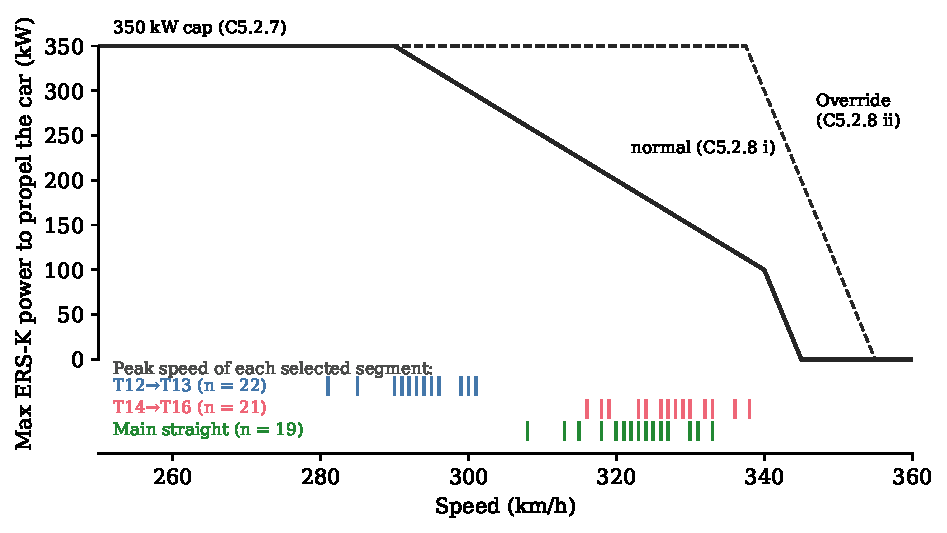
\includegraphics[width=\textwidth]{fig_taper.pdf}
  \caption{Maximum MGU-K power used to propel the car vs speed, FIA 2026 Technical Regulations Section C, Issue 12 \citep{fia2026c}: C5.2.8\,i (solid) and Override C5.2.8\,ii (dashed), both capped at 350~kW by C5.2.7. Ticks show the peak speed of each selected segment at Suzuka 2026: T12$\to$T13 281--301~km/h, T14$\to$T16 316--338~km/h, main straight 308--333~km/h.}
  \label{fig:taper}
\end{figure}

\subsection{Why clipping occurs}

A car accelerates while its propulsive power exceeds the power needed to overcome drag and other resistances. It slows down when the propulsive power falls below that need. If the electrical contribution is reduced or stops, the car can lose speed while the driver holds full throttle. This can happen through the taper, or because the energy store is not deploying. Energy is limited too. The ERS-K may harvest at most 8.5~MJ per lap, and at some events the FIA may reduce this to no less than 5~MJ in qualifying (C5.2.10). The energy store's state of charge may vary by at most 4~MJ while the car is on track (C5.2.9).

We use \emph{clipping} to mean exactly the observable: speed falling within a full-throttle segment. Telemetry does not show the state of charge, so we cannot say which mechanism causes a given loss.

\subsection{Two periods of the 2026 season}

Rule amendments took effect from the Miami Grand Prix (round 4). We do not analyse what they changed. We use the date only to split the season into a pre-Miami period (3 sessions) and a post-Miami period (14 sessions), because data quality differs between the two (Section~\ref{sec:freeze}).

\FloatBarrier
% ---------------------------------------------------------------------------
\section{Data}

\subsection{Source and sessions}

Telemetry comes from FastF1~3.8.3 \citep{fastf1}. FastF1 serves the official live-timing car data (Speed, RPM, nGear, Throttle, Brake) and position data (X/Y). Brake values are cross-checked against the OpenF1 \var{car\_data} endpoint \citep{openf1}, which was available for every session used.

Seventeen 2026 qualifying sessions were held up to the Singapore Grand Prix (10 October 2026). The Bahrain and Saudi Arabian rounds were cancelled, and the Bahrain Grand Prix was held at Sepang. FastF1 has no corner positions for Madrid or Sepang \citep{fastf1issue692}, so no corner-labelled straights could be defined there. Madrid contributes no reportable straight, and Sepang contributes its main straight only. For 2025 we use the 15 qualifying sessions held at circuits that were also raced in 2026, matched by OpenF1 \var{circuit\_key}. Team-to-PU mappings come from \citet{therace2026engines} for 2026 and \citet{si2025engines} for 2025.

\subsection{Validation of distance}

Following \citet{bopaiah2021}, we checked each driver's fastest-lap distance at Suzuka 2026 against the official length of 5.807~km. Distance integrated from X/Y position erred by $-0.83$ to $-0.43$\% (mean $|\text{error}|$ 0.58\%). Distance from car-data speed had a mean $|\text{error}|$ of 1.48\% and a maximum of 7.37\%. For comparison, \citet{bopaiah2021} report a mean error below 0.6\% and a maximum below 1.8\% for their reconstructed data. The large car-data errors come from frozen samples, described next.

\subsection{Frozen samples}
\label{sec:freeze}

Car data sometimes freeze: Speed, RPM and gear stay constant while the car keeps moving. On the 2026 Suzuka pole lap, car data froze at 189~km/h for 25.8~s. The same freezes appear in OpenF1, so they originate upstream of FastF1. Freezes are much more common in some sessions than in others (Figure~\ref{fig:freeze}). Mean freeze share on push laps was 7.0\% before Miami and 0.2\% from Miami onwards, and in 2025 it ranged from 0.00 to 0.06\% per session. Segments that overlap a freeze are dropped. The cleaning rules use documented sentinel values only and are given in full in Appendix~\ref{app:cleaning}.

\begin{figure}[tbp]
  \centering
  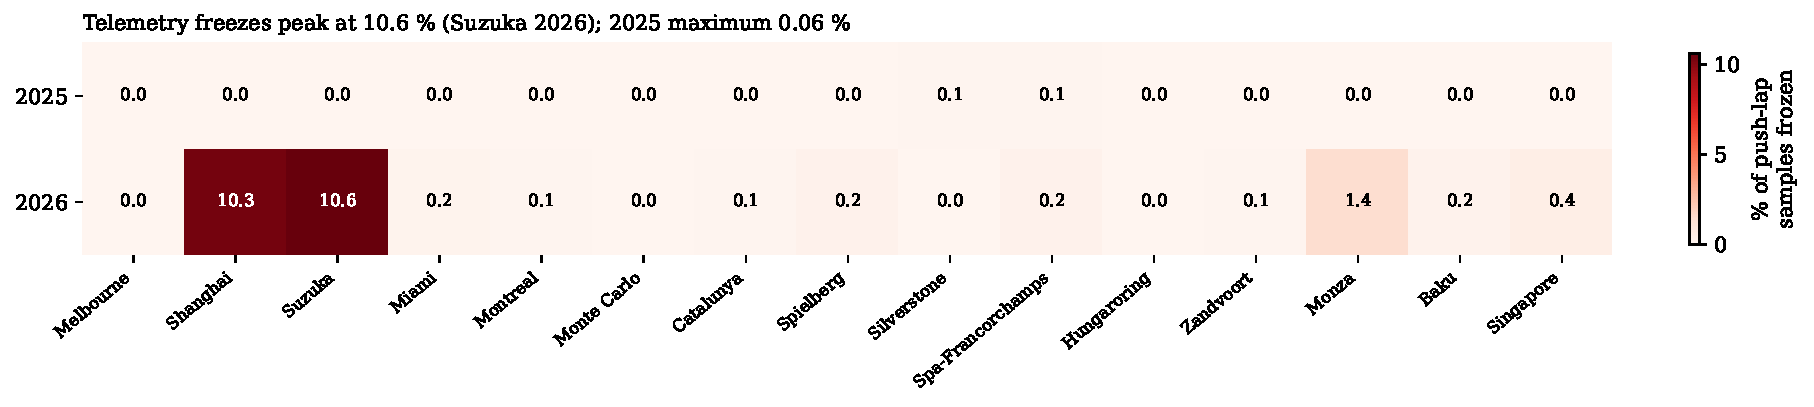
\includegraphics[width=\textwidth]{fig_regs_freeze_calendar.pdf}
  \caption{Freeze share (\% of push-lap car-data samples) per paired circuit (2026 calendar order) and year. 2025 range 0.00--0.06\%; 2026 range 0.00--10.60\%. Circuits above 1\% in 2026: Shanghai, Suzuka, Monza.}
  \label{fig:freeze}
\end{figure}

\subsection{Laps, segments and straights}

\emph{Push laps} are laps not involving the pit lane, within 107\% of the session's fastest lap, and not deleted by the stewards (FastF1 \var{pick\_wo\_box}, \var{pick\_quicklaps}, \var{pick\_not\_deleted}). We also reject laps whose speed is zero throughout, whose X/Y position is $(0,0)$ on any sample, or whose X/Y position is stationary throughout.

A \emph{full-throttle segment} is a run of samples with Throttle~$\ge 98$ and brake off (or unknown), at least 500~m long, with single-sample dips merged. Each segment is labelled by the corner it ends at, matched by X/Y position to FastF1's corner list (Figure~\ref{fig:map}). The main straight is stitched across the timing line and reported separately. For each driver and straight we keep one lap: the latest qualifying part with a clean segment first, then the fastest lap within it. A straight is \emph{reportable} in a session only if at least 10 drivers have a clean segment on it. This gives 41 reportable straights in 16 sessions (842 driver-straights): 8 straights before Miami and 33 from Miami onwards.

\begin{figure}[tbp]
  \centering
  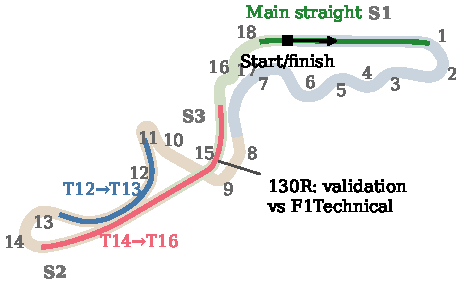
\includegraphics[width=0.48\textwidth]{fig_suzuka_map_a.pdf}
  \caption{Suzuka reference map, 2026: FIA sectors, corner numbers, start/finish with direction of travel, the three measured straights, and T15 (130R).}
  \label{fig:map}
\end{figure}

For 2025 vs 2026, a straight is matched if the same label exists at the same circuit in both years with at least 10 clean drivers each. This yields 39 matched straights at 15 circuits.

\FloatBarrier
% ---------------------------------------------------------------------------
\section{Method}

\subsection{Segment metrics}

For each selected segment, with distance $d$ from its start and length $L$:
\begin{itemize}
  \item \var{peak\_speed}: the maximum speed in the segment. Where several samples tie, the last one is used, so a plateau at top speed does not count as a loss.
  \item \var{vmax\_position} $= d_\text{peak}/L$: where the peak occurs, from 0 (segment start) to 1 (segment end). A value below 1 means the car reached its top speed before the driver lifted or braked.
  \item \var{clip\_delta} $=$ \var{peak\_speed} $-$ \var{end\_speed}: the \emph{speed lost after the peak} (km/h), measured up to the last full-throttle sample.
  \item \var{decel\_rate} $= 100\,\cdot$ \var{clip\_delta}$/(L - d_\text{peak})$: the speed lost per 100~m after the peak.
\end{itemize}
Speed is reported in integer km/h, so a drag-limited plateau can register a peak before the segment end with negligible loss. We therefore also report the share of drivers with \var{clip\_delta}~$\ge 2$~km/h. In the paired comparison, a straight \emph{shows no clipping} if its median \var{clip\_delta} is zero in both 2025 and 2026. Every other matched straight counts as a straight \emph{with clipping}.

\subsection{Aggregation}

Each plotted value is aggregated as follows.
\begin{itemize}
  \item \textbf{Peak position and speed loss, 2026} (Section~\ref{sec:res-peak}): raw values, one point per driver-straight. The split at the taper onset uses each driver-straight's own peak speed.
  \item \textbf{PU comparison, 2026} (Section~\ref{sec:res-pu}): for each straight in each session, we subtract the straight's mean over all clean drivers from each driver's value (\emph{centering}). We then pool driver-straights by PU and report median and IQR. Centering removes effects common to all cars on a straight, including gradient. The split by regime assigns a whole straight by its median peak speed.
  \item \textbf{2025 vs 2026, speed signature} (Section~\ref{sec:res-years}, Figure~\ref{fig:signature}): medians and IQR over all driver-straights in a year.
  \item \textbf{2025 vs 2026, per straight} (Section~\ref{sec:res-years}, Figures~\ref{fig:dumbbell} and~\ref{fig:maps}, Table~\ref{tab:paired}): for each matched straight and year, we take the median over drivers (one lap each). We then take the difference 2026~$-$~2025 per straight, and the median and IQR of that difference across straights.
\end{itemize}
2026 is pooled across PUs in the year comparison because the PU differences in the season were small (Section~\ref{sec:res-pu}). That is not proof that there are none.

\subsection{Robustness checks}
\label{sec:robust}

We used two checks on the paired comparison. First, we checked whether a straight's median segment end point moved more than 50~m between years, using position data, which could indicate a changed braking point or label. Second, we excluded sessions with rain recorded in FastF1 weather data.

\FloatBarrier
% ---------------------------------------------------------------------------
\section{Results}
\label{sec:results}

\subsection{2026 cars usually peak before the end of the straight}
\label{sec:res-peak}

In 2026 qualifying, most cars reach their peak speed before the end of the full-throttle segment and then lose speed while still at full throttle. Of the 842 driver-straights, 86\% peak before the segment end, with a median \var{vmax\_position} of 0.76 (Figure~\ref{fig:vmax}). \citet{therace2026fix} describes 2026 cars peaking earlier on a straight than earlier cars; the 2026 data alone cannot test that comparison, which Section~\ref{sec:res-years} makes with 2025 data.

\begin{figure}[bp]% bottom/page only: a top float here lands above the Results heading
  \centering
  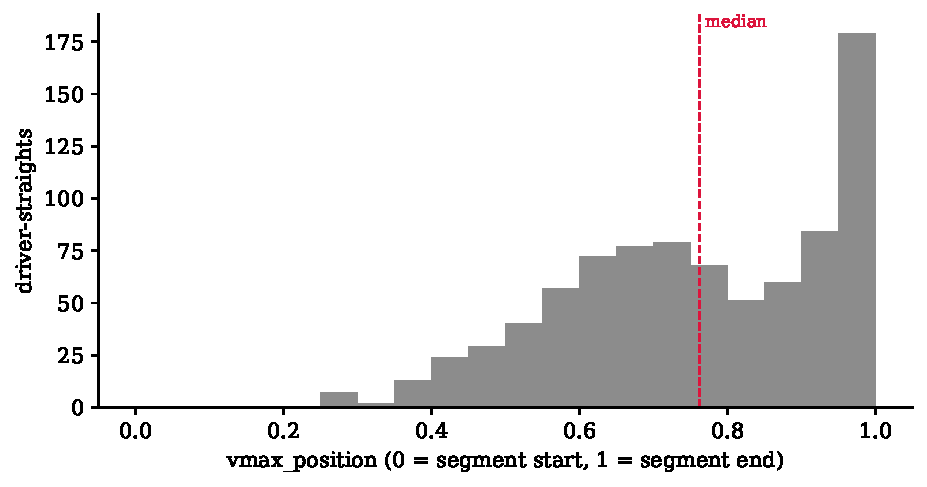
\includegraphics[width=0.48\textwidth]{fig_season_vmax_position.pdf}
  \caption{Where on the straight the peak speed occurs (\var{vmax\_position}), all 842 driver-straights on 41 reportable straights: 86\% peak before the segment end; median 0.76 (dashed).}
  \label{fig:vmax}
\end{figure}

The size of the loss after the peak does not rise uniformly with peak speed (Figure~\ref{fig:scatter}). The median loss is \emph{higher} below the taper onset than above it: 13.0~km/h for the 106 driver-straights that peak below 290~km/h, against 11.0~km/h for the 736 that peak at or above it. Below the onset the taper does not limit power. Most of these segments include corners taken flat out, where cars lose speed from drag and cornering load whatever the power limit. Above the onset, loss increases with peak speed (Spearman $\rho = 0.36$). This pattern is consistent with the speed-dependent C5.2.8 limit, but it is not evidence that the limit causes it. \textbf{Peak speed is confounded with straight length}: longer straights allow higher peak speeds and also more distance over which to lose speed. Circuit is confounded with both. These are raw, uncentered values.

\begin{figure}[tbp]
  \centering
  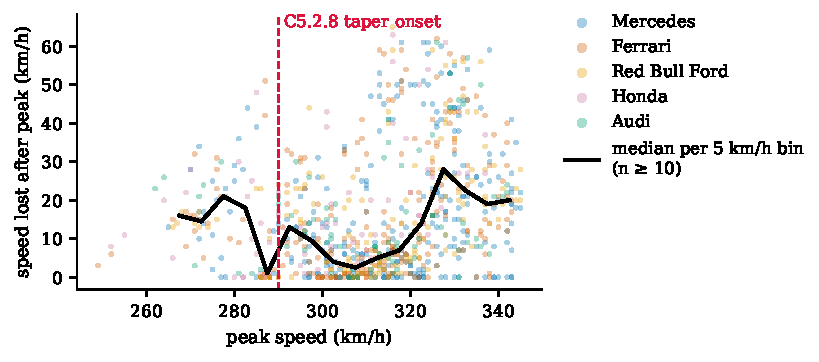
\includegraphics[width=\textwidth]{fig_season_peak_vs_clip.pdf}
  \caption{Speed lost after peak (\var{clip\_delta}) vs peak speed, one point per driver-straight on 41 reportable straights, coloured by PU. The black line is the median per 5~km/h bin, drawn only for bins with at least 10 driver-straights (3 sparser bins with 8 points in total are omitted from the line). Dashed: C5.2.8 taper onset (290~km/h). Straight length and circuit are confounded with peak speed.}
  \label{fig:scatter}
\end{figure}

\subsection{PU differences are about as large as teammate differences}
\label{sec:res-pu}

Once each straight's mean is removed, the spread between PU manufacturers is about the same as the spread between teammates. The PU medians of centered \var{clip\_delta} range from $-0.9$~km/h (Mercedes) to $+1.1$~km/h (Honda), a span of 2.1~km/h; teammates on the same straight differ by a median 2.0~km/h (IQR 1.0--4.0, 408 pairs). Team medians within a PU span up to 3.8~km/h, and the PU medians of centered \var{decel\_rate} range from $-0.49$ to $0.29$~km/h per 100~m (Figure~\ref{fig:pu}).

Splitting by regime gives similar results. Here each straight is assigned by its median peak speed, so the counts differ from the per-driver-straight split in Section~\ref{sec:res-peak}. On the 5 straights with median peak below 290~km/h (88 driver-straights), PU medians range from $-0.4$ to $2.9$~km/h. On the 36 straights at or above 290~km/h (754 driver-straights), they range from $-0.9$ to $2.4$~km/h. With one or two cars per team and one lap per driver, these numbers do not rank the PUs.

\begin{figure}[tbp]
  \centering
  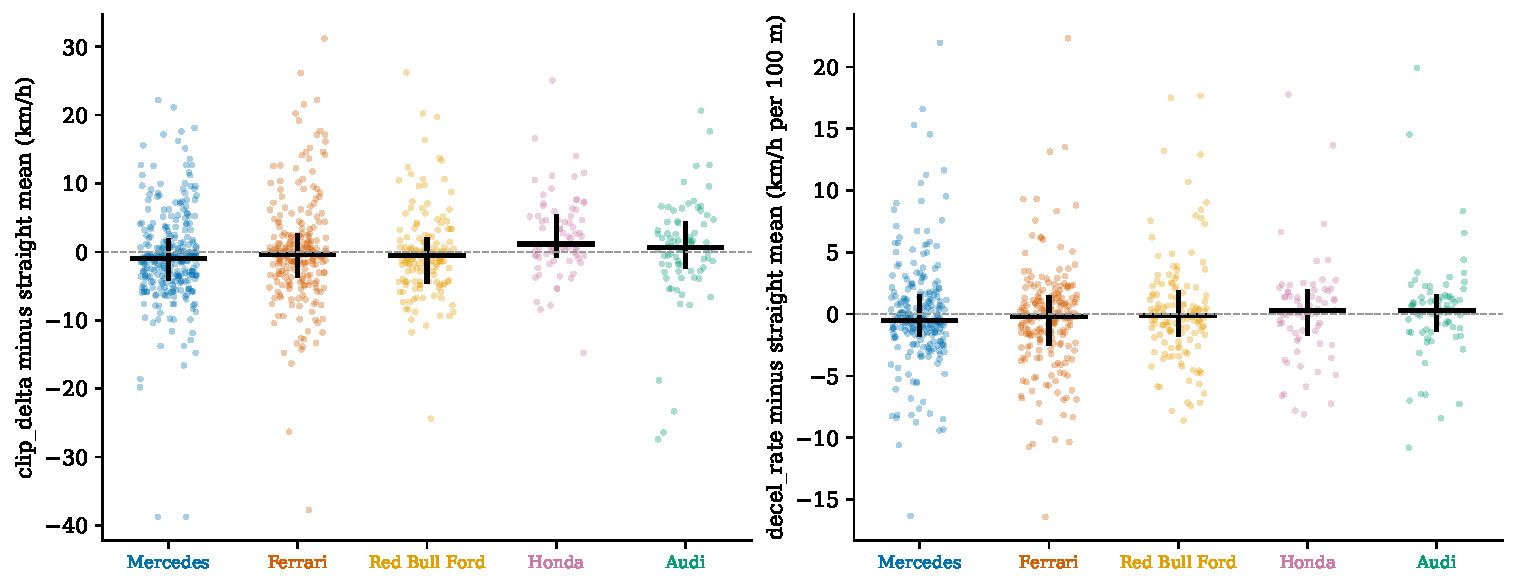
\includegraphics[width=\textwidth]{fig_season_centered_by_pu.pdf}
  \caption{Centered \var{clip\_delta} (left) and \var{decel\_rate} (right) per PU across 41 reportable straights in 16 sessions. Dots are driver-straights, the black bar is the median and the black line the IQR; 0 is the straight mean.}
  \label{fig:pu}
\end{figure}

\subsection{Every straight that clips does so earlier and harder in 2026}
\label{sec:res-years}

On all 33 matched straights with clipping, 2026 cars peak earlier and lose more speed after the peak than 2025 cars did on the same straight. The other 6 matched straights show no clipping in either year.

\paragraph{Speed signature.} Pooled over all matched straights, the 2026 speed profile rises faster and fades before the end of the segment (Figure~\ref{fig:signature}). Taken over all driver-straights, the median peak position is 1.00 in 2025 and 0.77 in 2026. Table~\ref{tab:paired} gives 0.99 for 2025 instead, because it is the median of the per-straight medians. The 2026 median curve lies above the 2025 curve from the segment start to 0.84 of its length, meaning a faster early gain relative to peak speed; the gap is 0.025 of peak speed at the start. The 2026 curve then falls below, ending at 96.4\% of peak speed against 100.0\% in 2025. This is a descriptive comparison and involves no statistical test.

\begin{figure}[tbp]
  \centering
  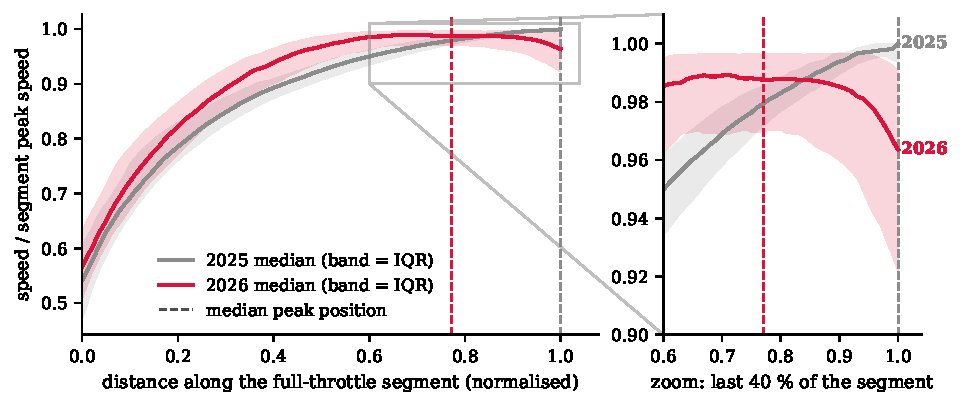
\includegraphics[width=\textwidth]{fig_regs_speed_signature.pdf}
  \caption{Speed signature of the 39 matched straights. Each driver-straight is resampled to normalised distance (0 = segment start, 1 = end), with speed divided by its segment peak. Line = median, band = IQR across driver-straights (762 in 2025, 801 in 2026). Dashed = median peak position over driver-straights (1.00 in 2025, 0.77 in 2026). Right panel: zoom on 0.6--1.0 of the segment (descriptive comparison; no statistical test).}
  \label{fig:signature}
\end{figure}

\paragraph{Straight by straight.} The shift holds on each clipped straight individually, not only on the pooled profile (Figure~\ref{fig:dumbbell}, Table~\ref{tab:paired}). Across the 33, the peak moved towards the start by a median 0.20 of the straight (range 0.01 to 0.59). Speed lost after the peak grew by a median 10.5~km/h (range 1.0 to 50.5). The smallest changes count the same as the largest: Monza T4 ($-0.01$, $+2.0$~km/h) and the Baku main straight ($-0.01$, $+1.0$~km/h). Some segments include corners taken flat out, where speed falls even in 2025 because of drag and cornering load; the paired design compares each straight with itself. The year difference reflects the whole 2026 package (PU, aerodynamics and the Straight-Line Mode wings), not any single rule.

\begin{figure}[tbp]
  \centering
  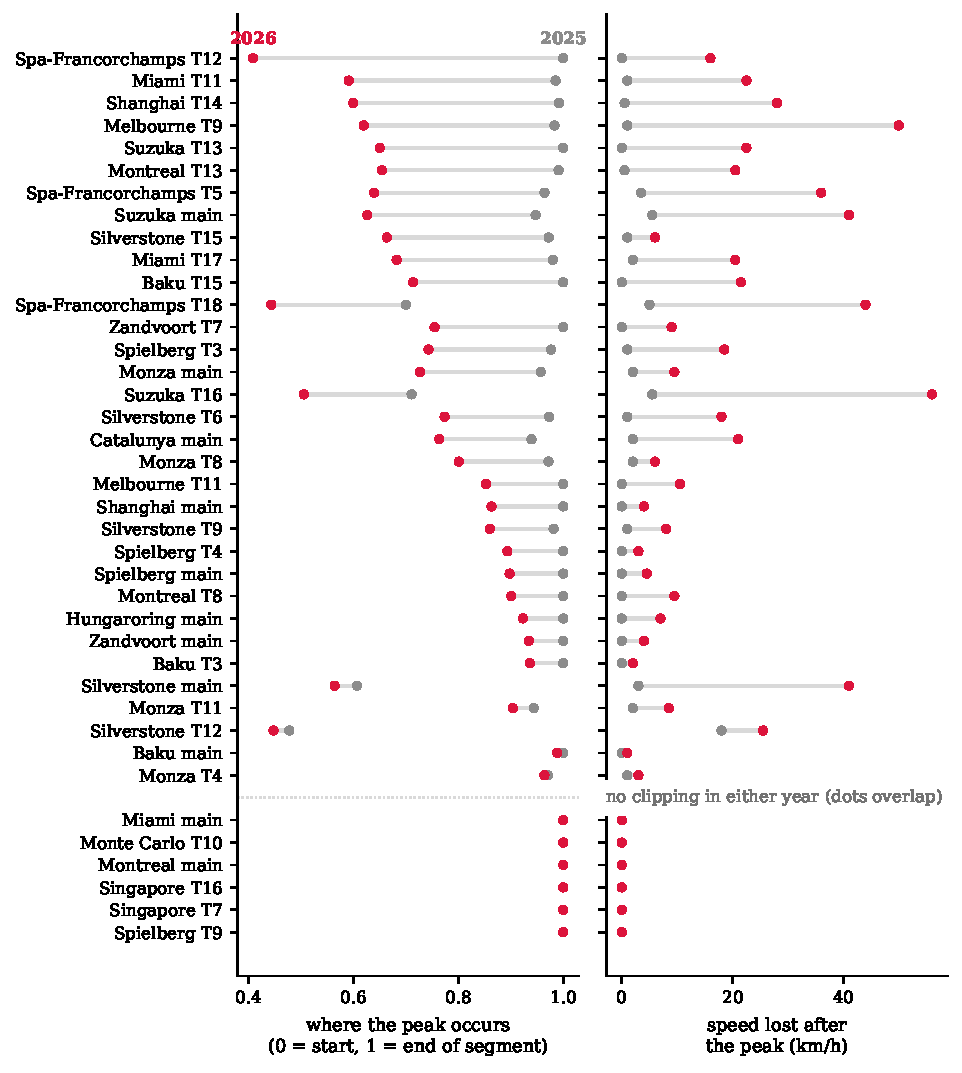
\includegraphics[width=\textwidth]{fig_regs_dumbbell.pdf}
  \caption{Each matched straight, 2025 (grey) and 2026 (accent) joined by a line. Each dot is the median across drivers on that straight in that year, one lap per driver, from 13--20 drivers in 2025 and 11--22 in 2026. Straights with clipping (33) are sorted by how far the peak moved; the 6 without clipping in either year are at the bottom, where the dots overlap. Showing paired data individually follows \citet{weissgerber2015}.}
  \label{fig:dumbbell}
\end{figure}

\begin{table}[tbp]
  \centering
  \caption{Paired difference 2026 $-$ 2025 per straight across 39 matched straights: median of the per-straight medians in each year, median and IQR of the difference across straights, and share of straights where 2026 is higher. ``Peak before end'' and ``loss $\ge$ 2~km/h'' are the shares of drivers on a straight.}
  \label{tab:paired}
  \small
  \begin{tabular}{lrrrr}
    \toprule
    Measure & Median 2025 & Median 2026 & Median diff.\ (IQR) & 2026 $>$ 2025 \\
    \midrule
    \var{vmax\_position} & 0.99 & 0.77 & $-0.15$ ($-0.29$ to $-0.04$) & 0\% \\
    \var{clip\_delta} (km/h) & 0.50 & 9.50 & $+7.50$ ($+3.50$ to $+20.75$) & 85\% \\
    Peak before end & 0.50 & 1.00 & $+0.31$ ($+0.10$ to $+0.51$) & 87\% \\
    Loss $\ge$ 2~km/h & 0.25 & 1.00 & $+0.40$ ($+0.16$ to $+0.68$) & 87\% \\
    \bottomrule
  \end{tabular}

  \medskip
  \begin{minipage}{0.92\textwidth}
    \footnotesize\textit{Note.} ``Peak before end'' rises on more straights (87\%) than median \var{clip\_delta} does (85\%). Because speed is reported in integer km/h, a driver on a drag-limited plateau can register a peak before the end with no measurable loss. On straights without clipping, the share of drivers peaking before the end can therefore rise while the median loss stays at zero. At the Montreal main straight, for example, the share rose from 0.05 to 0.36 while the median \var{clip\_delta} was 0 in both years.
  \end{minipage}
\end{table}

\paragraph{Robustness.} The result does not depend on the two checks in Section~\ref{sec:robust}. Median segment end points moved 0--32~m between years (median 12~m), so no straight crossed the 50~m flag. Rain fell during qualifying at Baku in 2025 and at Montreal and Zandvoort in 2026. Excluding those sessions leaves 31 matched straights: on all 26 with clipping, 2026 cars peak earlier and lose more speed, and the other 5 show no clipping in either year. The median \var{clip\_delta} difference stays at $+7.50$~km/h.

\paragraph{Suzuka.} A single circuit shows the pattern on the track map (Figure~\ref{fig:maps}). On the fastest freeze-free push lap in each year, the maximum speed lost after a segment's peak is 10~km/h in 2025 (VER, lap 16) and 50~km/h in 2026 (PIA, lap 16). Each map shows one lap, so it illustrates the pattern rather than measuring it.

\begin{figure}[tbp]
  \centering
  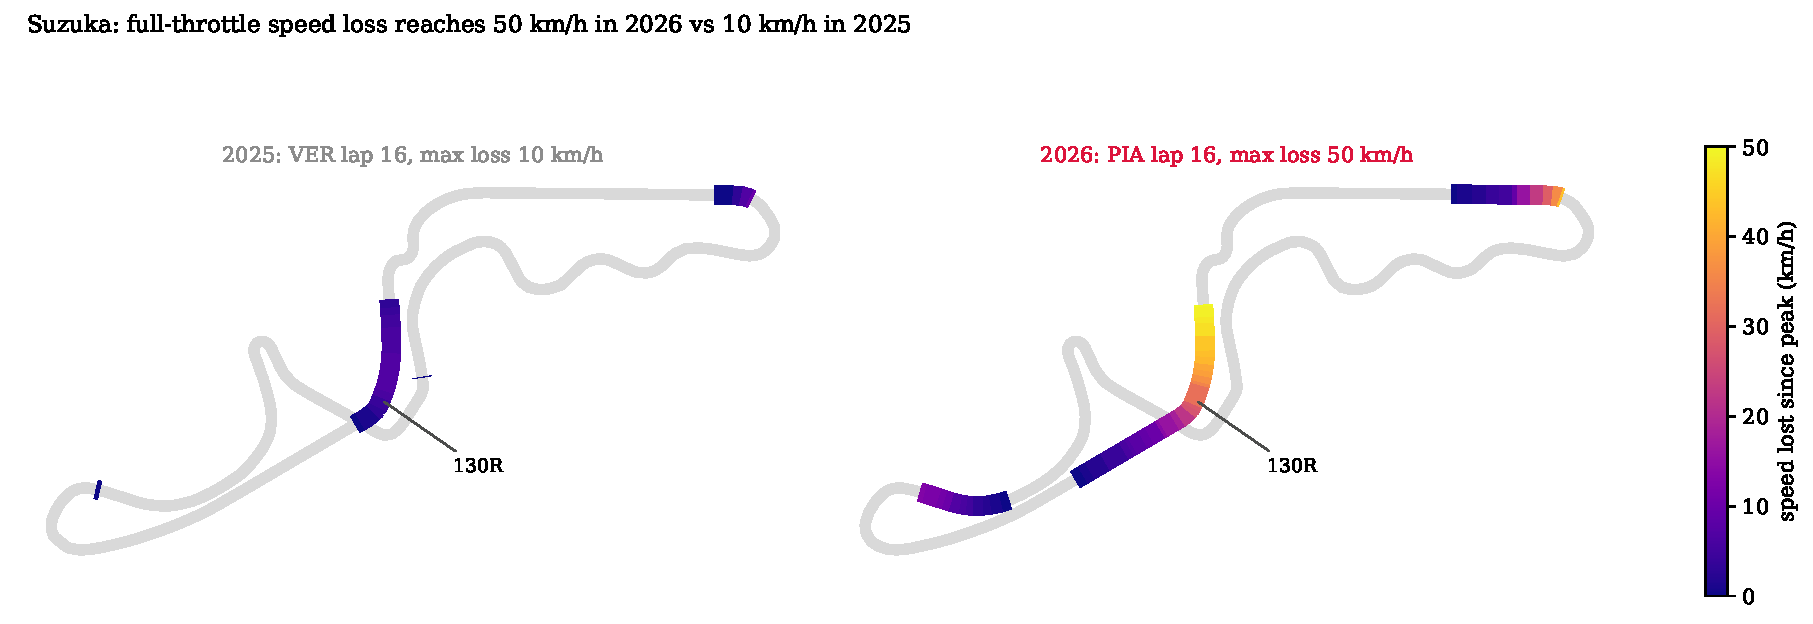
\includegraphics[width=\textwidth]{fig_regs_suzuka_maps.pdf}
  \caption{Suzuka clipping maps on one colour scale, fastest freeze-free push lap per year (2025 VER lap 16, maximum 10~km/h; 2026 PIA lap 16, maximum 50~km/h). Colour = speed lost since the segment's peak, from the peak to the segment end; grey = outside full-throttle segments or before the peak.}
  \label{fig:maps}
\end{figure}

\FloatBarrier
% ---------------------------------------------------------------------------
\section{Discussion}

Taken together, the three findings describe a behaviour that is widespread, new and common to the field. Most 2026 driver-straights peak before the end of the full-throttle segment, and above the taper onset the speed lost after the peak tends to grow with peak speed. The spread between PU manufacturers is no larger than the spread between teammates, so at this resolution the data do not separate the manufacturers. Against 2025, every matched straight that clips produces an earlier peak and a larger loss. The pattern is therefore better described as a property of the 2026 cars as a group than of any one manufacturer, although one or two cars per team cannot rule out smaller PU differences.

Compared with \citet{bopaiah2021}, the approach trades depth for breadth. They studied one qualifying session, combined broadcast-derived speed traces with a full-vehicle simulation, and could therefore estimate the energy recovered by the MGU-K. We have no energy model. Instead we measure one observable across a season, with a matched set of 2025 sessions, every exclusion logged, and cleaning rules fixed on one event before the season was run. The approaches are complementary: a single-session model can explain how a car uses its energy, and a season-wide measurement shows how general a pattern is.

The causal question, how much of the loss is due to the C5.2.8 taper and how much to energy limits or to team and driver choices, cannot be answered from public telemetry. It would require the energy store's state of charge, the ERS-K deployment power along the lap, the energy harvested per lap against the C5.2.10 limit, and the use of Override Mode. With those channels, taper-limited and energy-limited speed loss could be separated straight by straight.

\FloatBarrier
% ---------------------------------------------------------------------------
\section{Limitations}

\begin{itemize}
  \item \textbf{Descriptive only.} We fit no models and run no tests. No difference reported here is an estimated effect.
  \item \textbf{Confounding.}
  \begin{itemize}
    \item Peak speed is confounded with straight length and circuit (Section~\ref{sec:res-peak}).
    \item The split before and after Miami is confounded with circuit, because no circuit appears in both periods. Pre-Miami data quality was also worse (mean freeze share 7.0\% vs 0.2\%). We therefore do not interpret the pre/post difference: median \var{clip\_delta} was 26.0~km/h on 8 pre-Miami straights and 9.0~km/h on 33 post-Miami straights. We do not analyse the content of the Miami amendments.
  \end{itemize}
  \item \textbf{Whole-package comparison.} The 2025 vs 2026 difference reflects every change between the two cars, not the C5.2.8 taper alone.
  \item \textbf{Unobserved state.} Telemetry has no state of charge, deployment or energy limit, so we cannot attribute a given speed loss to the taper, to the energy limits, or to driver choice.
  \item \textbf{Sample.} There are one or two cars per team and one lap per driver per straight. Madrid and Sepang have no corner-labelled straights.
  \item \textbf{Measurement.} Speed is reported in integer km/h. Freezes remove more data in some sessions (up to 10.6\% at Suzuka 2026). The \var{JumpFlag} robustness check (Appendix~\ref{app:cleaning}) was run for Suzuka only, where 1 of 62 selected segments was flagged and excluding it changed mean \var{clip\_delta} per straight by at most 0.4~km/h.
  \item \textbf{Rules on 2025 data.} The \var{JumpFlag} bound is derived from 2026 values and is not interpreted for 2025.
\end{itemize}

\FloatBarrier
% ---------------------------------------------------------------------------
\section{Conclusion}

Public telemetry, cleaned with documented sentinel values only, is sufficient to measure full-throttle speed loss across a Formula One season. In 2026 qualifying, losing speed before the end of a straight is the norm rather than the exception, it is not specific to one manufacturer, and on the same straights it is new relative to 2025. Why it happens is a separate question: separating the C5.2.8 taper from the energy limits requires channels that are not public.

\FloatBarrier
\section*{Data and code availability}
The pipeline (\texttt{flatout.py}) and notebooks are available at \url{https://github.com/see7ien/Flat-Out}. All numbers in this paper are taken from the notebook outputs.

% ---------------------------------------------------------------------------
\appendix
\renewcommand{\thefigure}{A\arabic{figure}}
\renewcommand{\theHfigure}{A\arabic{figure}}
\setcounter{figure}{0}
\section{Cleaning rules}
\label{app:cleaning}

We use only documented sentinel values and tune no thresholds:
\begin{itemize}
  \item[(a)] A run of unchanged Speed, RPM and gear that contains \var{Throttle}~$=104$ is a freeze, plus a one-sample buffer on each side. FastF1 documents the value 104 for stationary cars \citep{fastf1}; we observe it during running. Segments that overlap a freeze are dropped.
  \item[(b)] OpenF1 \var{brake}~$=104$ means the brake state is unknown. It does not end a full-throttle segment and is trimmed from the segment's end. OpenF1 \var{brake}~$=100$ is taken as genuine braking.
  \item[(c)] A single-step speed increase of at least 5~km/h beyond what 800~kW could produce for a 700~kg car is flagged (\var{JumpFlag}), not removed. Results are reported with and without flagged segments, in the spirit of a multiverse analysis \citep{steegen2016}.
\end{itemize}
We also tested a Speed/RPM ratio check \citep[sec.~6.4]{segers2014}. It did not separate stale from updating speed, so it is used only as a diagnostic. Figure~\ref{fig:freezemap} shows where the flagged samples fall on the Suzuka lap in 2026.

\begin{figure}[tbp]
  \centering
  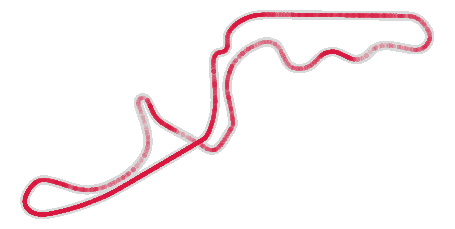
\includegraphics[width=0.48\textwidth]{fig_suzuka_map_b.pdf}
  \caption{Locations of 3,940 flagged car-data samples (including one-sample buffers) on 75 of 108 push laps, Suzuka 2026.}
  \label{fig:freezemap}
\end{figure}

\FloatBarrier
\bibliographystyle{plainnat}
\bibliography{refs}

\end{document}
